\documentclass[11pt,a4paper]{article}
\usepackage[margin=1in]{geometry}
\usepackage{graphicx}
\usepackage{booktabs}
\usepackage{array}
\usepackage{url}
\usepackage[hidelinks]{hyperref}
\graphicspath{{../figures/}}

\title{Macromate: Pakistani Food Recognition and Nutrition Logging\\Deliverable 1 Technical Report}
\author{Mohid Israr (24L-2510)\\Adnan Zaka (24i-2537)\\Hassan Mehmood (24L-2559)}
\date{}

\begin{document}
\maketitle

\begin{abstract}
Macromate is a proposed image-assisted nutrition logger for eight Pakistani-style dishes. This report documents the completed first deliverable: source tracking, validation, cleaning, image preparation, exploratory analysis, nutrition-reference checks, and a reproducible train/validation/test split. The checked-in collection contains 400 images (50 per dish). All 400 passed input validation; no exact or threshold-defined near duplicates were found; four file-size outliers were retained. A fixed-seed, group-aware split produced 280 training, 64 validation, and 56 reserved test images, with no detected group or near-duplicate leakage. Two complete pipeline runs produced 424 identical generated files. These findings establish a reproducible data baseline, not recognition accuracy: CLIP training, held-out evaluation, and the application have not yet been implemented. Original provider export archives and README files are unavailable, and a second human review of all labels remains pending.
\end{abstract}

\section{Problem and Users}
Macromate aims to make nutrition logging easier for adults who track Pakistani meals for general fitness. A user will upload a photo of one main dish, confirm or correct the suggested label, and enter a serving size. The system will calculate approximate calories and macronutrients from a documented reference. Recipe variation means the result is an estimate.

\section{Why AI Is Needed}
Food photos differ in angle, lighting, background, and recipe appearance. Simple fixed rules cannot reliably distinguish dishes such as chicken biryani and chicken pulao. We plan to measure the accuracy of pretrained CLIP on selected Pakistani dishes, fine-tune a small part of its image encoder using labeled photos, and compare both versions on the same held-out test set. Nutrition multiplication is not treated as an AI task.

\section{Scope and Labels}
The initial labels are chicken biryani, chicken pulao, chicken karahi, daal, nihari, haleem, samosa, and chapati. The final list depends on the image and nutrition data audit. Mixed plates, automatic portion estimation, and medical advice are outside the initial scope.

\section{Data Collection}
The selected collection contains 400 images, 50 per dish, from four Roboflow Universe datasets: combined-dataset (Rafias Workspace, 258 selected), IndianFoodRecog (EnVisionAI, 64), samosa (new, 50), and Bangladeshi Food Classification2 (NSN, 28). The original classes and their mapping to our eight dish labels are recorded in \texttt{data/sources.csv} and \texttt{data/metadata.csv}. The source records include the version URL, access date, export format, uploader-stated CC~BY~4.0 license, transformation notes and archive SHA-256. Each image record includes its original path, selected label, source-photo group and file SHA-256. The repository-derived summaries in \texttt{evidence/} verify source counts and the hashes of the 400 committed images. They are derived from the checked-in manifests and images, not from the original export archives. The original exports and provider README files were not preserved, so the recorded archive hashes and uploader license statements cannot be independently rechecked from this checkout. All selected labels still require the planned second human review.

\section{Cleaning and Preprocessing}

\subsection{Input validation}
The raw manifest \texttt{data/metadata.csv} lists 400 images, 50 for each of the eight dishes, collected from four public Roboflow datasets released under CC~BY~4.0 (Table~\ref{tab:sources}). The script \texttt{clean\_data.py} checks required columns, missing values, supported dish names, source identifiers, duplicate IDs, whether each file exists, and whether it can be decoded. The original records are never edited; cleaned outputs go to \texttt{data/processed/} and every removed record would be logged with its reason in \texttt{exclusions.csv}.

\begin{table}[h]
\centering
\begin{tabular}{lp{5.6cm}r}
\hline
Source ID & Used for & Images \\ \hline
RF\_COMBINED (Rafias Workspace) & biryani, karahi, nihari, haleem, pulao (22), daal (36) & 258 \\
RF\_CHAPATI (EnVisionAI) & chapati, daal (14) & 64 \\
RF\_SAMOSA & samosa & 50 \\
RF\_NSN (Bangladeshi Food Classification) & pulao (28) & 28 \\ \hline
\end{tabular}
\caption{Image sources in the cleaned collection (all CC~BY~4.0 as stated by the uploaders).}
\label{tab:sources}
\end{table}

All 400 records passed validation: no missing values, unknown labels, unknown sources, duplicate IDs, missing files or unreadable images. No exact duplicates (SHA-256) and no images with conflicting labels were found, so the cleaned set also contains 400 images. This is largely because the collector had already removed augmentation copies and kept at most one representative per source photo before delivery.

\subsection{Duplicates and outliers}
Resized or re-compressed copies are detected with a 64-bit perceptual (difference) hash; pairs within 6 bits would be written to \texttt{near\_duplicate\_pairs.csv} for human review rather than deleted automatically. No pair was that close: the closest pair differs by 10 bits. Six groups of images that derive from the same original photograph (shared \texttt{source\_photo\_group}) are kept together in the split described below.

Image outliers are flagged but not removed: shorter side below 224 px, aspect ratio above 3:1, files under 5~KB, and width, height or file size beyond three interquartile ranges. Four images were flagged, all because their file size (about 100--111~KB) exceeded the upper fence of 96~KB (two chapati and two samosa images). They are ordinary photographs with more detail, so they are retained and documented. No image is smaller than 224 px.

Nutrition values (\texttt{nutrition.csv}) are checked for missing or negative values, macronutrients summing to more than 100~g per 100~g, energy above 900~kcal per 100~g, a missing source or recipe assumption, and disagreement of more than 25\% between reported energy and the 4/4/9 kcal-per-gram estimate from the macronutrients. All eight dish rows passed; all values are per 100~g.

\subsection{Normalisation and encoding}
Following the official CLIP preprocessing \cite{clipcode}, each image is converted to RGB (after EXIF rotation), resized so its shorter side is 224 px with bicubic interpolation, and centre-cropped to $224\times224$. The pipeline saves these RGB images as PNG files and records paths and labels in \texttt{clip\_manifest.csv}. It does \emph{not} save normalised tensors. A model loader must scale pixels to $[0,1]$ and normalise them per channel with CLIP's mean $(0.4815, 0.4578, 0.4082)$ and standard deviation $(0.2686, 0.2613, 0.2758)$. These pretrained-model constants are not recomputed from our data. The preprocessing audit applied that transformation in memory: across 400 images the pixel mean changed from $(0.623, 0.522, 0.395)$ to $(0.529, 0.245, -0.047)$ and the standard deviation from $(0.276, 0.279, 0.311)$ to $(1.027, 1.067, 1.126)$, with normalised values between $-1.79$ and $2.15$. Nonzero means reflect this collection's colour distribution and are not evidence of a processing error.

Dish names are encoded as stable integer IDs in a fixed order: chicken biryani 0, chicken pulao 1, chicken karahi 2, daal 3, nihari 4, haleem 5, samosa 6, chapati 7 (saved in \texttt{label\_map.json}). Nutrition stays in per-100~g units and is deliberately not scaled, because the app calculation (value per 100~g $\times$ grams $/\,100$) needs the original units.

\subsection{Train/validation/test split and reproducibility}
\texttt{split\_data.py} divides each dish 70/15/15 with a fixed random seed (42): 35 training, 8 validation and 7 test images per dish, giving 280, 64 and 56 images in total (Figure~\ref{fig:split}). Near-duplicate and same-photo images are placed in one subset together. The leakage checks found no group spanning two subsets and no near-duplicate pair across subsets (smallest cross-subset hash distance: 10 bits). The test subset is reserved for the final comparison of zero-shot and fine-tuned CLIP; no CLIP training is performed in this deliverable.

\begin{figure}[h]
\centering
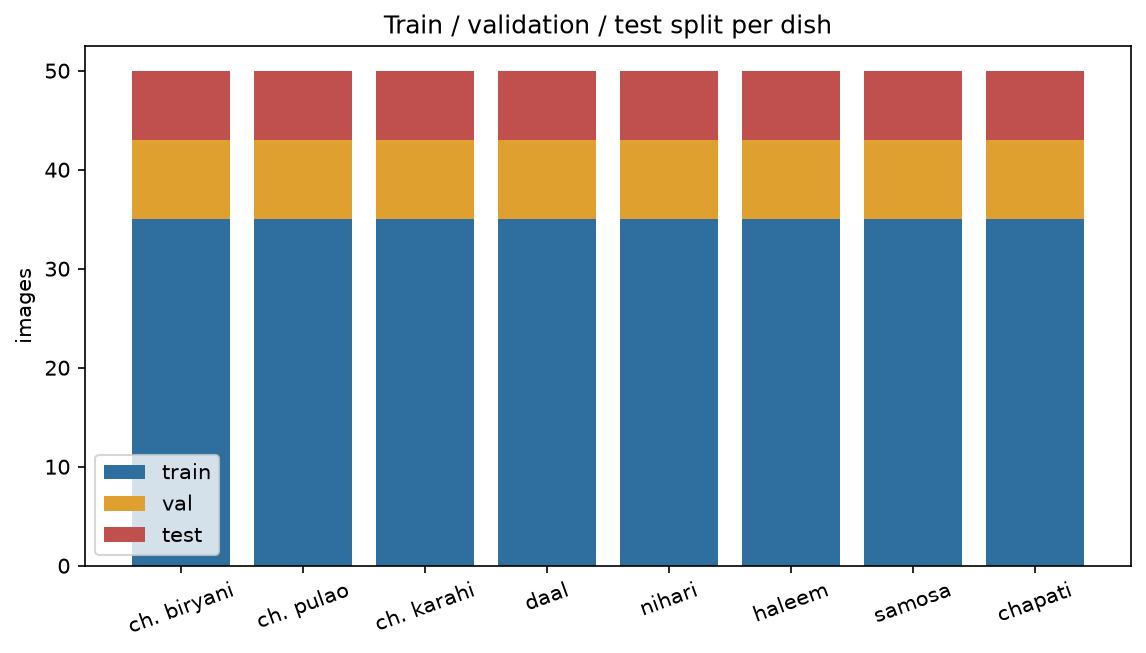
\includegraphics[width=0.85\textwidth]{../figures/split_distribution.png}
\caption{Train/validation/test counts per dish.}
\label{fig:split}
\end{figure}

\texttt{verify\_reproducible.py} runs the source audit, cleaning, preprocessing, split and EDA twice; it checks output completeness and compares SHA-256 hashes of all generated CSV, JSON and PNG outputs. For the current dataset, all 424 checked files were identical on the second run. The machine-readable comparison can be regenerated as \texttt{data/processed/reproducibility\_check.json}.

\section{Initial Data Exploration}

Figure~\ref{fig:counts} shows the collection is perfectly balanced at 50 images per dish. Because the collector had already screened the raw downloads, the raw and cleaned counts are the same, and the manifest has no missing values in any column. This meets the minimum size we set, but is below the 60--100 images per dish proposed, so test accuracy will be estimated from only 7 photographs per dish.

\begin{figure}[h]
\centering
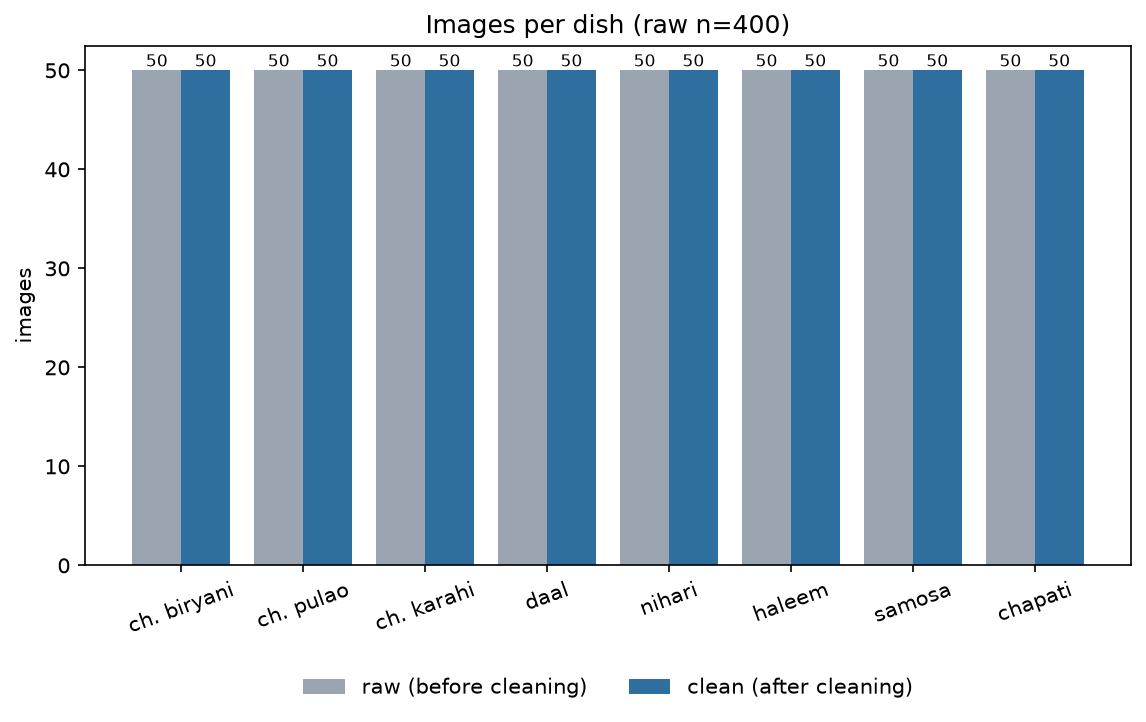
\includegraphics[width=0.85\textwidth]{../figures/raw_class_counts.png}
\caption{Raw and cleaned image counts per dish.}
\label{fig:counts}
\end{figure}

Figure~\ref{fig:samples} shows four photographs per dish. They vary in plate, background, camera angle and lighting, as intended. Some are visually close: biryani and pulao are both rice dishes, and the pulao class mixes 22 ``chicken pulao'' images with 28 Bangladeshi ``morog polao'' images, which the collector mapped to chicken pulao and disclosed as a regional difference. The daal class likewise mixes dal tadka, maash daal and mixed dal, while the nutrition reference is for one daal recipe.

\begin{figure}[h]
\centering
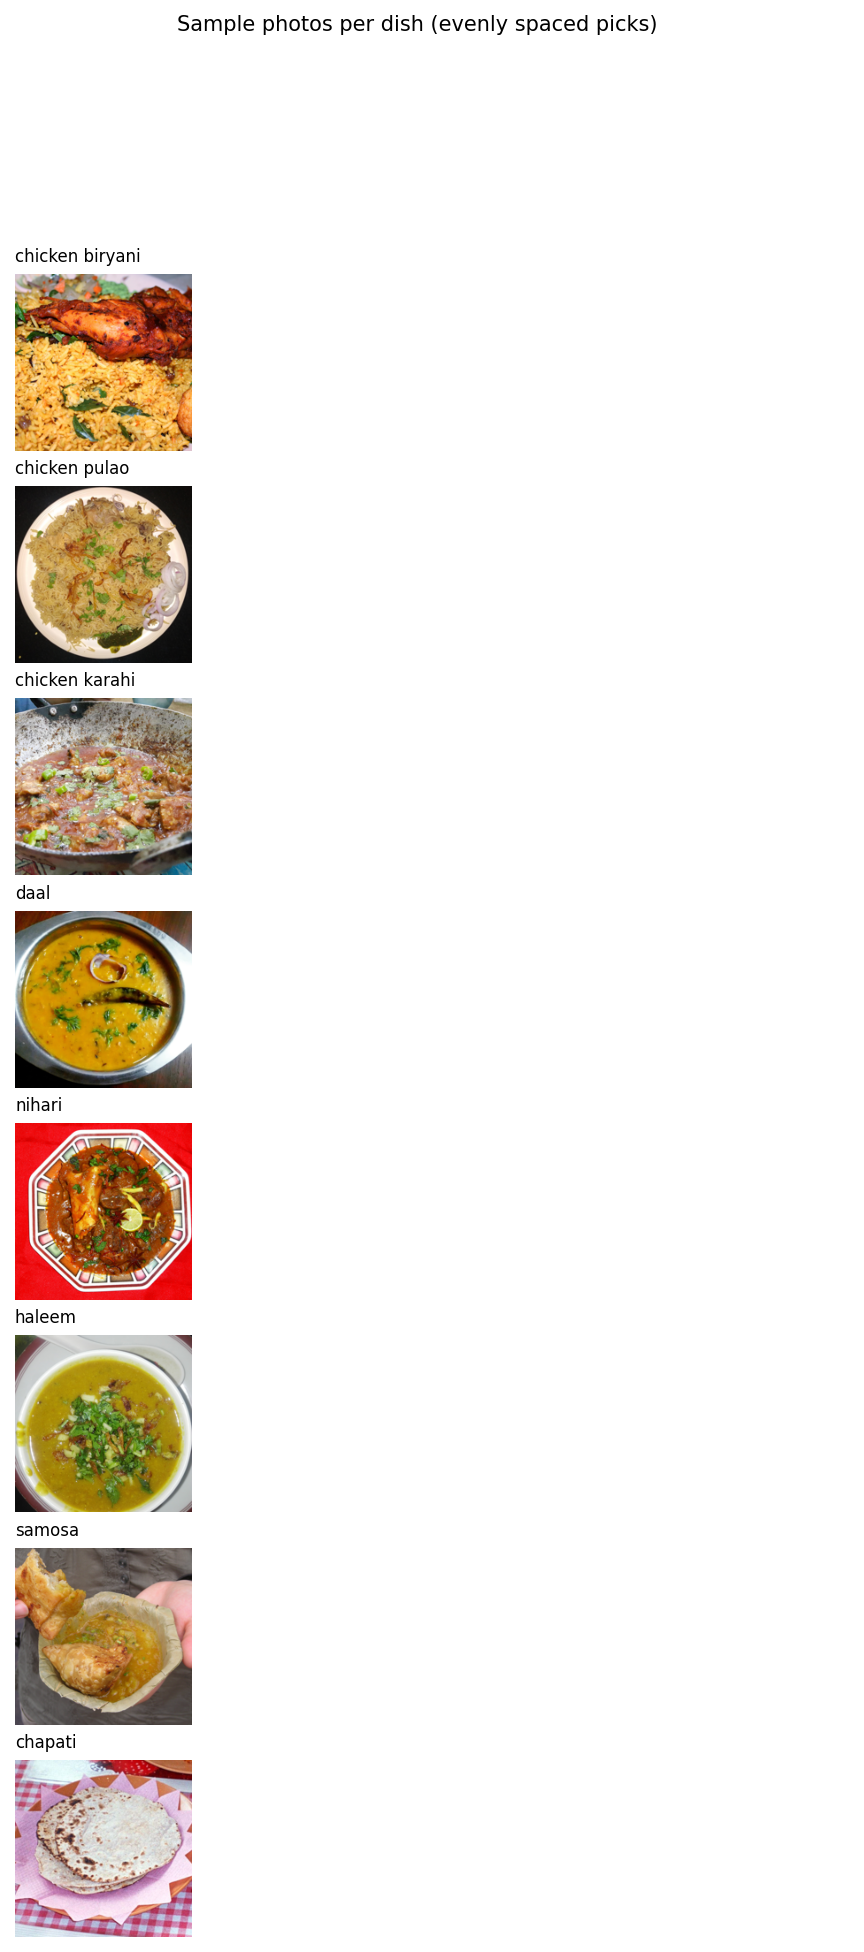
\includegraphics[width=0.55\textwidth]{../figures/sample_images.png}
\caption{Sample photographs for each dish. Images are from the Roboflow Universe datasets by EnVisionAI, Rafias Workspace, NSN and ``new'' (see Table~\ref{tab:sources}), used under CC~BY~4.0; they are not modified apart from resizing for display.}
\label{fig:samples}
\end{figure}

Figure~\ref{fig:sizes} shows image sizes. Every image is square, at 256, 432 or 640 pixels per side, because the dataset providers resized them by stretching; the aspect ratio is therefore 1.0 for all images, and photographs with other proportions appear distorted. File sizes range from 7 to 111~KB. Figure~\ref{fig:source} reveals a more important pattern: image size and source depend strongly on the dish. All chapati and samosa images are 640~px and come from single sources, while biryani, karahi, nihari and haleem are 432~px, and 28 of the pulao images are 256~px. A model could partly learn a source's image style or resolution instead of the dish. CLIP rescales everything to 224~px, which reduces but does not remove this risk, so the results must be interpreted with this in mind.

\begin{figure}[h]
\centering
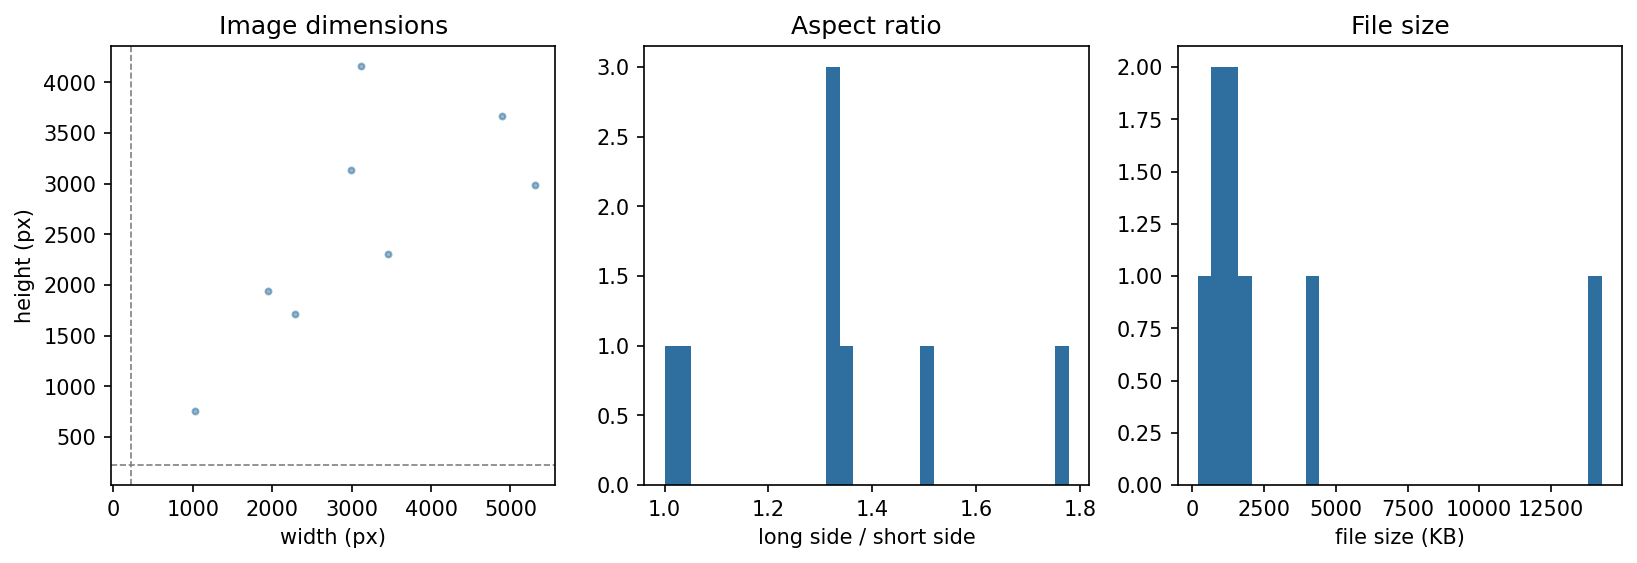
\includegraphics[width=\textwidth]{../figures/image_size_distribution.png}
\caption{Image dimensions (bubble size shows the number of images), aspect ratio and file size.}
\label{fig:sizes}
\end{figure}

\begin{figure}[h]
\centering
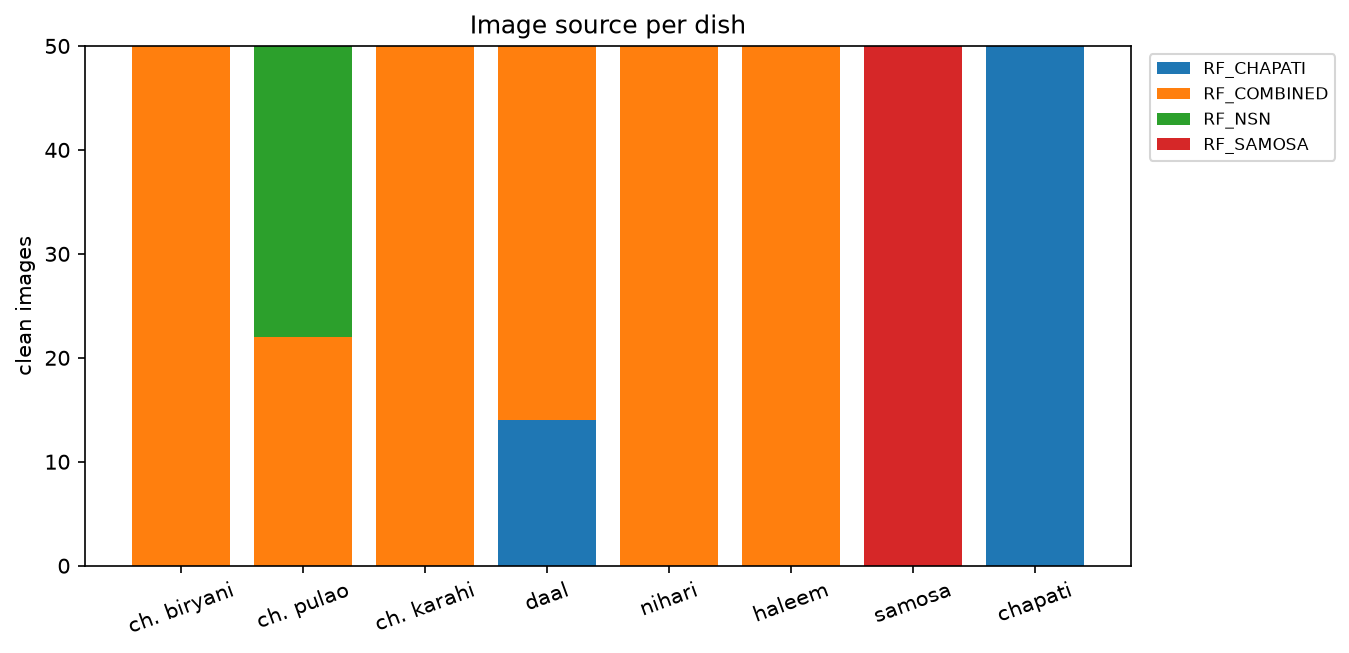
\includegraphics[width=0.85\textwidth]{../figures/class_by_source.png}
\caption{Image source for each dish.}
\label{fig:source}
\end{figure}

Figure~\ref{fig:corr} shows correlations between image-level features. Brightness is almost perfectly correlated with the mean green channel (0.99) and strongly with red (0.92) and blue (0.93), as expected, and file size correlates with width (0.73) because larger images have more bytes. Width, height and aspect ratio are not independent features here: height always equals width and the aspect ratio is constant, so only one of them is shown. We create no extra numeric features from these values.

\begin{figure}[h]
\centering
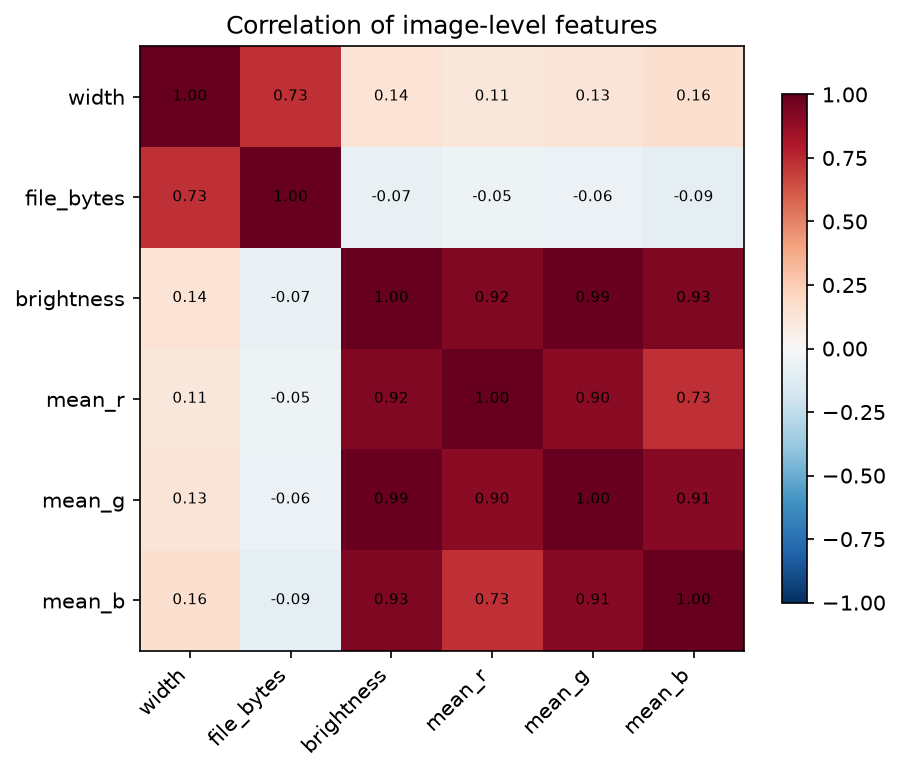
\includegraphics[width=0.7\textwidth]{../figures/feature_correlation.png}
\caption{Correlation of image-level features.}
\label{fig:corr}
\end{figure}

Figure~\ref{fig:nutrition} compares the reference nutrition per 100~g. Chapati and samosa are the most energy-dense (259 and 220~kcal), while chicken biryani and chicken karahi are the lowest (about 107 and 105~kcal). These values come from specific recipes and products, so they are documented proxies, not exact values for every photographed dish.

\begin{figure}[h]
\centering
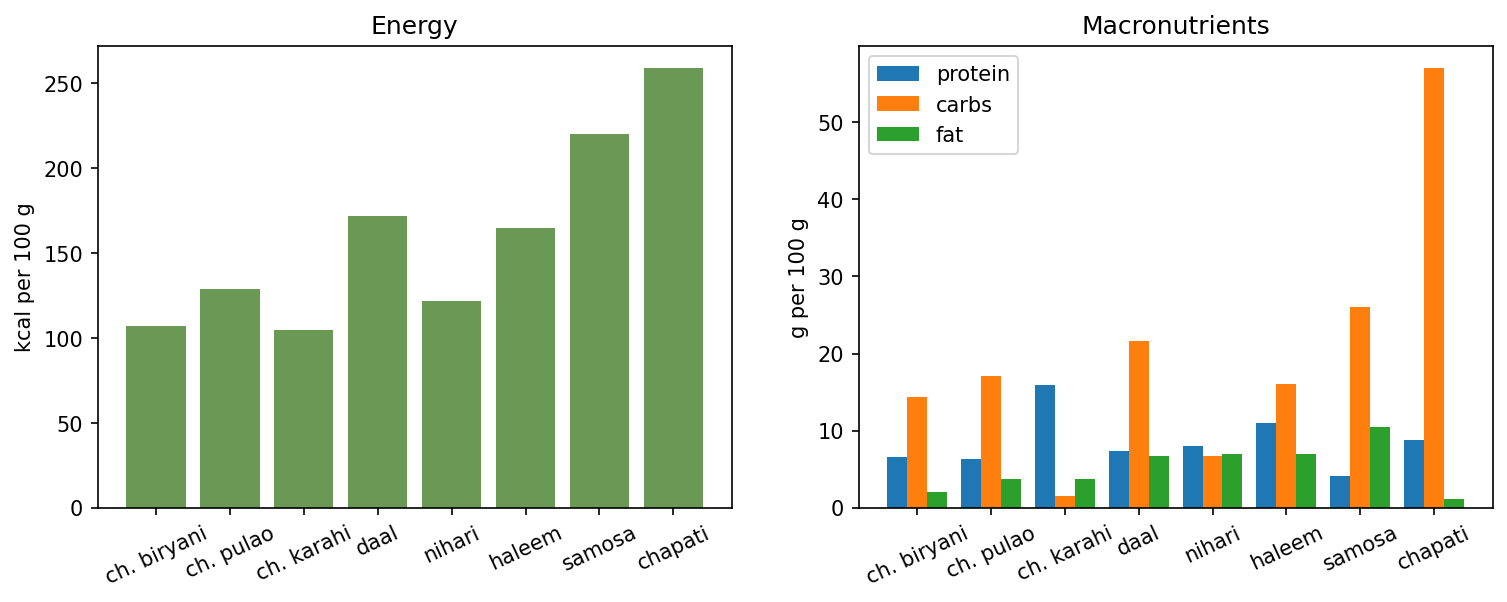
\includegraphics[width=\textwidth]{../figures/nutrition_macros.png}
\caption{Reference energy and macronutrients per 100~g for each dish.}
\label{fig:nutrition}
\end{figure}

\paragraph{Limits.} All 400 labels come from the source datasets' own classes and an AI-assisted contact-sheet screen; the second human review required by the project plan is still pending. The sources are largely Indian and Bangladeshi, so Pakistani appearance and recipes are only partly represented.

\section{Nutrition Calculation and Provenance}
The application will use a fixed per-100~g reference row for each confirmed dish. For a user-entered serving mass $m$ in grams and a nutrient value $n_{100}$ per 100~g, the displayed estimate is
\begin{equation}
n(m)=n_{100}\frac{m}{100}.
\end{equation}
This deterministic calculation requires user confirmation of the dish and serving mass; the image classifier will neither infer mass nor select ingredients. Table~\ref{tab:nutrition} gives the checked reference values. For example, 150~g of the selected chicken-biryani reference gives about 160~kcal, 9.9~g protein, 21.5~g carbohydrate, and 3.1~g fat. These numbers describe the reference recipe, not the photographed meal. Source URLs and recipe assumptions are recorded row by row in \texttt{data/nutrition.csv}; the daal, nihari, haleem, and samosa entries are explicit recipe or product proxies.

\begin{table}[ht]
\centering
\small
\begin{tabular}{lrrrr}
\toprule
Dish & kcal & Protein (g) & Carbohydrate (g) & Fat (g) \\
\midrule
Chicken biryani & 106.89 & 6.63 & 14.32 & 2.09 \\
Chicken pulao & 128.60 & 6.40 & 17.10 & 3.80 \\
Chicken karahi & 104.59 & 15.96 & 1.50 & 3.79 \\
Daal & 171.73 & 7.35 & 21.61 & 6.78 \\
Nihari & 121.88 & 8.01 & 6.72 & 7.04 \\
Haleem & 165.00 & 11.00 & 16.00 & 7.00 \\
Samosa & 220.00 & 4.10 & 26.00 & 10.50 \\
Chapati & 259.00 & 8.80 & 57.00 & 1.20 \\
\bottomrule
\end{tabular}
\caption{Audited reference values per 100~g; recipe variation is not represented.}
\label{tab:nutrition}
\end{table}

\section{Planned Recognition Experiment}
The proposal specifies a zero-shot CLIP baseline followed by partial fine-tuning of its image encoder while keeping the text encoder fixed \cite{clip}. Each class will receive a consistently worded prompt, such as ``a photo of Pakistani chicken biryani''. The eight text embeddings and an image embedding will be compared using the same similarity head in both conditions. Prompt wording and training settings may be chosen using the validation subset; the 56 test photographs must remain untouched until the final comparison. Both conditions will use the same test images, label order, and preprocessing. Planned measures are top-1 and top-3 accuracy, per-dish accuracy, and a confusion matrix, with particular attention to chicken biryani versus chicken pulao. An accuracy estimate from only seven test images per class will be imprecise, so raw counts should accompany percentages. No recognition result is claimed in this report.

\section{Reproducibility and Limitations}
The source audit, cleaning, preprocessing, split, and EDA are implemented as scripts under \texttt{data scripts/}. Their outputs include manifests, summaries, 400 prepared PNGs, and eight figures. Four regression tests cover relevant pipeline edge cases. A full two-run verification compared 424 generated outputs and found identical hashes. The repository thus supports replay of the \emph{checked-in collection} and its preparation steps.

Several constraints remain material to any future accuracy or product claim. The original Roboflow archives and provider README files are unavailable, so recorded archive hashes, export transformations, and uploader license statements cannot be revalidated against original packages; the four summaries in \texttt{evidence/} are derived from repository files. The second independent human label review is pending for all 400 images. The collection has 50 images per class, below the proposal's 60--100 target, and only seven test images per class. Dish and dataset source are correlated, which can inflate apparent performance through source-specific backgrounds, stretching, or resolution. Some mapped classes include regional or recipe variants, and single-reference nutrition values cannot capture ingredients, oil, or serving composition. Deployment and advice features should therefore wait for label review, external-photo evaluation, and explicit uncertainty handling.

\section{Conclusion}
The first deliverable establishes a balanced, audited and reproducible dataset pipeline with a reserved test split and documented nutrition references. It does not yet establish that the proposed classifier distinguishes the eight dishes or that its nutrition estimates match individual meals. The next technical milestone is independent label review followed by the preregistered zero-shot and fine-tuned CLIP comparison on the untouched split.

\begin{thebibliography}{9}
\bibitem{proposal} Macromate team, \emph{Macromate Project Proposal}, project repository, 2026.
\bibitem{clip} A. Radford et al., ``Learning Transferable Visual Models From Natural Language Supervision,'' \emph{Proceedings of the 38th International Conference on Machine Learning}, 2021. \url{https://proceedings.mlr.press/v139/radford21a.html}.
\bibitem{clipcode} OpenAI, \emph{CLIP reference preprocessing and implementation}. \url{https://github.com/openai/CLIP/blob/main/clip/clip.py}.
\end{thebibliography}

\end{document}
